\documentclass{article}
\usepackage[utf8]{inputenc}
\usepackage{graphicx}

\title{VE489 Homework 5}
\author{Wei Yinuo 520370910103}
\date{July 2023}

\begin{document}

\maketitle
\begin{enumerate}
    \item 
    Optimality principle.
    
    \item
    \begin{enumerate}
        \item In distance vector routing, routers keep a table called a routing table which holds details about the metric (distance) and the next-hop direction to reach each destination network. These routing tables store information like the distance between routers or networks, which can be measured using factors such as the number of routers crossed (hop count), bandwidth, delay, or other appropriate measurements.
        
        \item
        The routing path setup begins at the destination node. 
        
        \item
        The Bellman-Ford algorithm is suitable for distance vector routing because it effectively calculates optimal paths and distances in a network. By exchanging routing information between neighboring routers, distance vector routing algorithms can utilize the iterative nature of the Bellman-Ford algorithm. It allows routers to update their routing tables based on received information, enabling the determination of the best routes. The algorithm's decentralized nature and ability to find the shortest path from a single source node align well with the distributed nature of distance vector routing.
        
        \item
        Distance vector routing provides several advantages. It is known for its simplicity, making it easy to implement and understand. With lower processing and memory requirements, it is suitable for routers with limited capabilities, making it efficient in small to medium-sized networks. Configuration is straightforward as routers exchange routing tables, facilitating updates across the network. Distance vector algorithms incorporate loop prevention mechanisms like hop count limitations, split horizon, and poison reverse, ensuring stable and efficient routing.
        \newline
        Once convergence is achieved, distance vector routing offers stable routing paths, beneficial for networks with relatively static topologies. It also allows flexibility in choosing metrics for calculating distances, enabling optimization based on specific network requirements. Additionally, distance vector routing scales well in smaller networks and hierarchical structures, where routers exchange information within their respective regions.
        
        \item
        Convergence can be slower, potentially leading to longer periods of suboptimal routing. It may also face challenges in scaling to larger networks due to its limited view of the network topology. Advanced routing protocols, such as link-state protocols (e.g., OSPF) and hybrid protocols (e.g., EIGRP), have been developed to address these limitations while offering enhanced performance and scalability.
        
    \end{enumerate}
    Reference:
    Computer Networking: A Top-Down Approach, James F. Kurose, Keith W. Ross, 7th Edition
    \newline
    "Computer Networks", Andrew S. Tanenbaum and David J. Wetherall

    \item
    Please see Figure \ref{fig:frog}.
    \begin{figure}
        \centering
        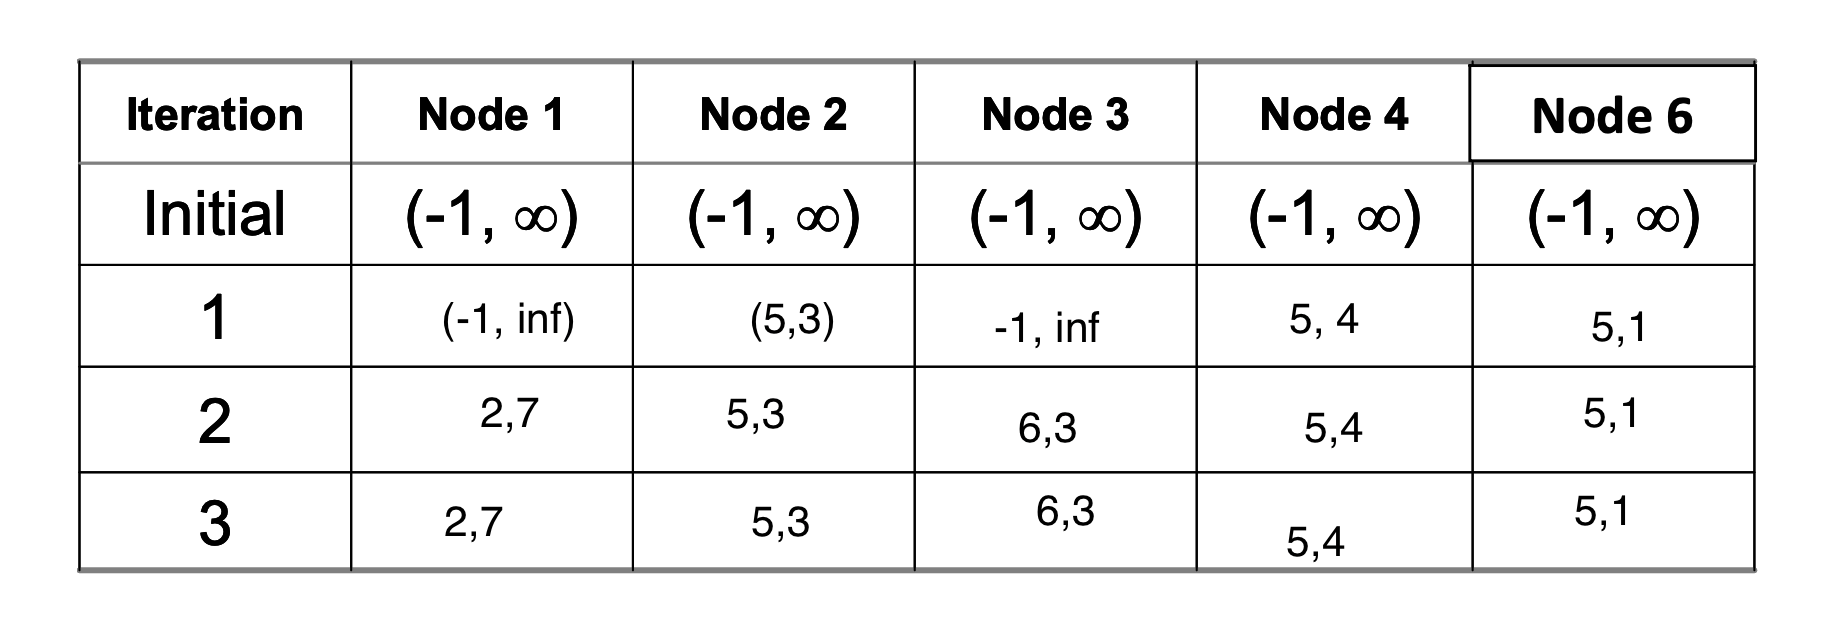
\includegraphics[width=0.9\textwidth]{h5ex3.png}
        \caption{\label{fig:frog}Problem 3}
    \end{figure}
    
    \item
    \begin{enumerate}
        \item Link state routing is a centralized scheme. 
        \item
        Dijkstra's algorithm is followed in the link state routing.
        \item
        In link state routing, it is not necessary to include the entire routing path in the packet header. Instead, routers use their routing tables to determine the next hop for packet forwarding. Including the entire routing path would introduce unnecessary overhead and increase packet size. It is more efficient to rely on the routing table information at each router, which already contains the optimal paths to reach destinations. This approach ensures flexibility, scalability, and adaptability to dynamic network changes without the need to encode the entire routing path in the packet header.
        \item
        Pros of Link State Routing Protocol:
Link state routing protocols offer efficient and fast convergence due to their accurate and up-to-date network topology information. They prevent routing loops with mechanisms like split horizon and poison reverse. Scalability is achieved through hierarchical designs and area partitioning, reducing overhead. Flexibility in selecting metrics allows customization to meet specific network requirements.
\newline 
Cons of Link State Routing Protocol:
Link state protocols demand higher resource usage, consuming more memory and processing power than distance vector protocols. Their configuration and management can be complex. Frequent link state advertisement exchanges increase network overhead, and large networks may face scalability challenges. They rely on accurate information sharing, leaving them vulnerable to attacks like spoofing or malicious link state advertisements.
        
    \end{enumerate}
    
    \item
    The multiplexing and access mechanisms are crucial for regulating the flow of packet traffic. Queueing and scheduling are carefully considered at multiplexing points to ensure efficient utilization of network resources and deliver Quality of Service (QoS). The objective is to prioritize different types of traffic, including Fault-recovery packets, Real-time traffic, Enterprise (high-revenue) traffic, and high bandwidth traffic. This approach determines the relative performance offered to packets within a short time scale, enabling effective management of network traffic and meeting specific QoS requirements.
    \newline 
    To be specific, typical schemes include FIFO queueing, HOL priority queueing, earliest due date scheduling, fair queueing.
    
    \item
    Flow level is an ideal perspective of packet level control. Flow-level traffic management offers a broader perspective on traffic patterns, enabling the formulation of high-level strategies for managing various flow types. It establishes the overall guidelines and policies for traffic handling. On the other hand, packet-level traffic management operates at the granular level of individual packets, ensuring adherence to the flow-level policies for each packet within a flow. By collaborating, flow-level and packet-level traffic management optimize the handling of traffic, ensuring efficiency and effectiveness. The decisions made at the flow-level inform the packet-level management, enabling the processing of packets in accordance with the predefined policies. This collaborative approach leads to enhanced network performance and the delivery of QoS.
    
    \item
        Please see Figure \ref{fig:fro}.
    \begin{figure}
        \centering
        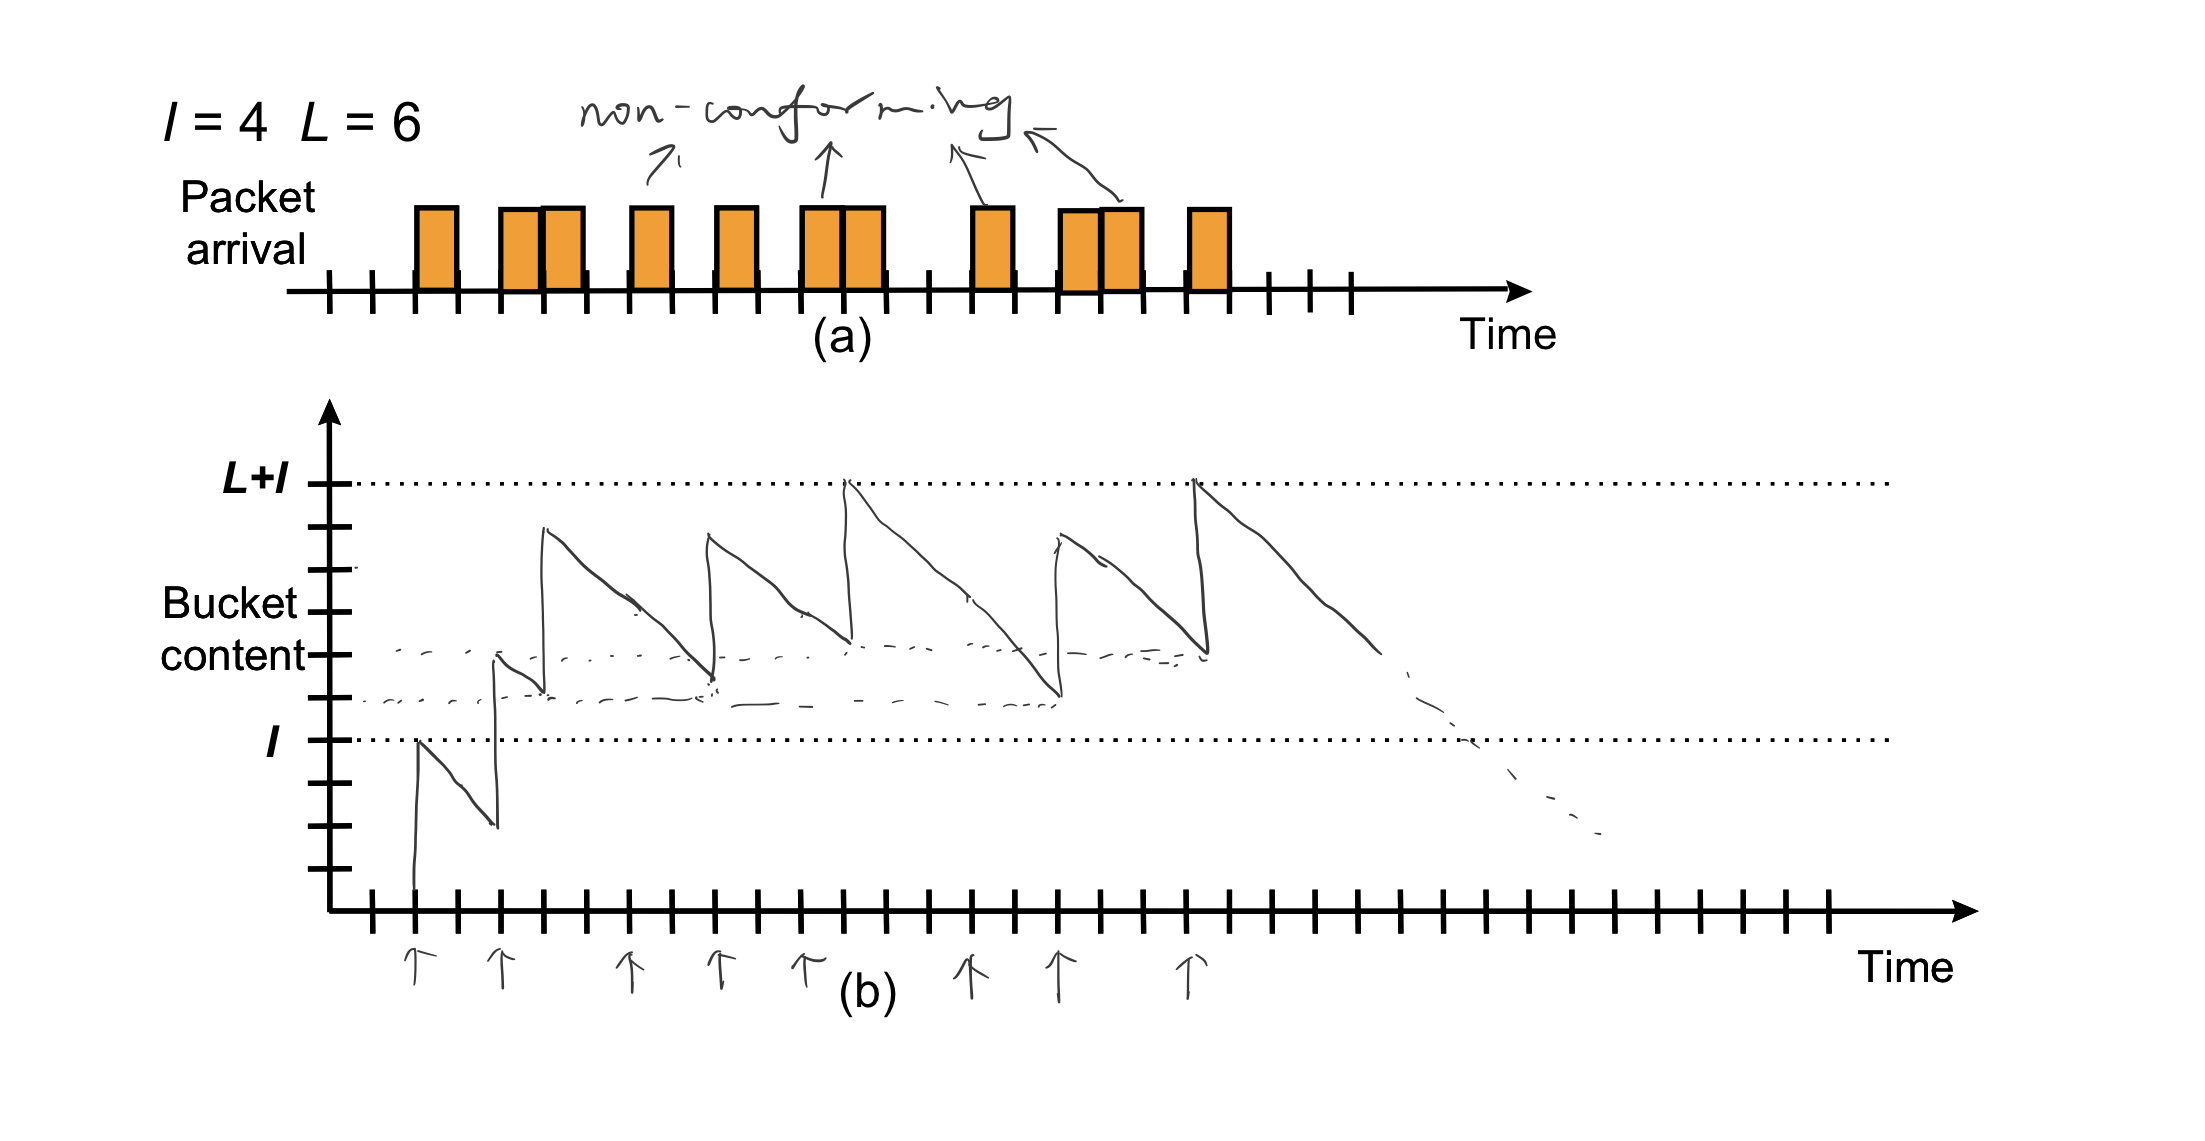
\includegraphics[width=0.9\textwidth]{h5ex7.jpg}
        \caption{\label{fig:fro}Problem 7}
    \end{figure}
    
    \item
    For token bucket, the leak rate changes, while leaky bucket does not. The leaky bucket algorithm smoothes out bursts of traffic by limiting the overall rate. In contrast, the token bucket algorithm allows for occasional bursts as long as there are sufficient tokens available. Leaky bucket can be used for entering the internet traffic and token bucket for exiting.
    
    
    
\end{enumerate}

\end{document}
